% This is samplepaper.tex, a sample chapter demonstrating the
% LLNCS macro package for Springer Computer Science proceedings;
% Version 2.20 of 2017/10/04
%
\documentclass[runningheads]{llncs}
%
\usepackage{helvet,times,courier}
\usepackage{graphicx}
\usepackage{changepage}
\usepackage{cite}
\usepackage{algorithm}
\usepackage{algpseudocode}
\usepackage{mathtools}
\usepackage{rotating}
\usepackage{caption}
\usepackage{url}
\usepackage{todonotes}
\usepackage[inline]{enumitem}
\usepackage{xspace}
\captionsetup[table]{skip=10pt}
\DeclarePairedDelimiter\ceil{\lceil}{\rceil}
% Used for displaying a sample figure. If possible, figure files should
% be included in EPS format.
%
% If you use the hyperref package, please uncomment the following line
% to display URLs in blue roman font according to Springer's eBook style:
% \renewcommand\UrlFont{\color{blue}\rmfamily}

\renewcommand{\algorithmicrequire}{\textbf{Input:}}
\algnewcommand{\To}{{\normalfont\bfseries to }}

\newcommand{\stest}{\textit{ST\_EST}\xspace}
\newcommand{\stmtwr}{\textit{ST\_MTWR}\xspace}
\newcommand{\stfifo}{\textit{ST\_FIFO}\xspace}

\newcommand{\wtest}{\textit{WT\_EST}\xspace}
\newcommand{\wtmtwr}{\textit{WT\_MTWR}\xspace}
\newcommand{\wtfifo}{\textit{WT\_FIFO}\xspace}

\begin{document}
%
\title{Decomposition-based Job-shop Scheduling with Constrained Clustering
\thanks{This work was partially funded by
KWF project 28472,
cms electronics GmbH,
FunderMax GmbH,
Hirsch Armbänder GmbH,
incubed IT GmbH,
Infineon Technologies Austria AG,
Isovolta AG,
Kostwein Holding GmbH, and
Privatstiftung Kärntner Sparkasse.}}%\thanks{Supported by organization x.}}
%
% \titlerunning{Decomposition-based JSP with Constrained Clustering}
% If the paper title is too long for the running head, you can set
% an abbreviated paper title here
%
\author{Mohammed M. S. El-Kholany\inst{1,3}\orcidID{0000-0002-1088-2081} \and
Konstantin Schekotihin\inst{1}\orcidID{0000-0002-0286-0958} \and
Martin Gebser\inst{1,2}\orcidID{0000-0002-8010-4752}}
%
\authorrunning{M. El-Kholany et al.}
% First names are abbreviated in the running head.
% If there are more than two authors, 'et al.' is used.
%
\institute{Alpen-Adria-Universität Klagenfurt, % Klagenfurt, 
Austria\\% 
% \email{\{mohammed.el-kholany, konstantin.schekotihin and martin.gebser\}@aau.at}%\\
%\url{http://www.springer.com/gp/computer-science/lncs}
\and
Technische Universität Graz, % Graz, 
Austria\\%
\and
% Faculty of Computers and Artificial Intelligence,
Cairo University, 
Egypt\\%
% \email{mgebser@ist.tugraz.at}
\email{firstname.lastname@aau.at}}
%
\maketitle              % typeset the header of the contribution
%
\begin{abstract}
Scheduling is a crucial problem appearing in various domains, such as manufacturing, transportation, or healthcare, where % . In most problem definitions, 
the goal is to schedule % a given set of 
given operations on available resources such that the operations are completed as soon as possible. Unfortunately, most scheduling problems cannot be solved efficiently, % Therefore, the 
so that research on suitable approximation methods is of primary importance.
%
This work introduces a novel approximation approach based on problem decomposition with data mining methodologies. We propose a constrained clustering algorithm to group operations into clusters, corresponding to time windows in which the operations must be scheduled. 
The decomposition process consists of two main phases. 
First, features are extracted, either from the problem itself or from solutions obtained by heuristic methods, to predict the execution sequence of operations on each resource.
% The first phase is to extract features to predict the sequence of operations on each resource. These features are extracted either from the problem itself or from solutions obtained by other heuristics.
The second phase % is to develop
deploys our constrained clustering algorithm to assign each operation into a time window. We then schedule the operations by time windows using Answer Set Programming. Evaluation results show that our proposed approach outperforms other heuristic schedulers in most cases, where incorporating features like \textit{Remaining Processing Time}, \textit{Machine Load}, and \textit{Earliest Starting Time} significantly improves the solution quality.

\keywords{Job-shop Scheduling  Problem \and Constrained Clustering \and Time Windows \and Answer Set Programming}
\end{abstract}
%
%
%
\section{Introduction}
Scheduling is one of the most crucial problems in various industrial, transportation, or healthcare applications
%\todo{add 1-2 citations for each application}
 \cite{pezzella2008genetic,chaudhry2016research,nouiri2018effective,demirbilek2019dynamically,schoenfelder2020nurse,wang2019routing,janakbhai2021blockchain}. 
%
Such applications result in different scheduling problem definitions, with the Job-shop Scheduling Problem (JSP) \cite{taillard1993benchmarks} being one if not the most well-known variant.
In JSP, operations of given jobs must be scheduled on available machines in an optimal way wrt.\ some predefined criteria. The latter include, for instance, minimization of makespan, i.e., the latest completion time of any job, or tardiness, i.e., the sum of delays over all jobs completed after their deadlines. 

However, JSP is an NP-hard combinatorial optimization problem \cite{garey1976complexity,SOTSKOV1995237} for which no efficient algorithms are known. Therefore, searching for an optimal solution with state-of-the-art solvers for Answer Set Programming (ASP), Mixed Integer Programming, or Constraint Programming \cite{meng2020mixed,coltep19a,el2020job,al2017job}
%\todo{cite at least 1 paper solving JSP with these methods} 
often takes too much computation time, even for seemingly small instances. Practical applications instead necessitate solving JSP instances of large scale with thousands of operations~\cite{zhang2010hybrid}.
As a result, much research work focuses on % the development of 
efficient methods for finding high-quality approximations of optimal schedules, including dispatching rules and other heuristic approaches~\cite{blackstone1982state} as well as stochastic optimization techniques \cite{DBLP:journals/informs/VaessensAL96,DBLP:journals/jim/CalisB15}.  
The main issue of these approaches is that they require manual parametrization for a particular scheduling problem, which is tedious and error-prone. For instance, adapting heuristic methods might involve the development of new dispatching rules or specific combinations of existing ones. Similarly, merely utilizing default parameters for stochastic techniques might lead to mediocre schedules.    
In view of these challenges, recent research interest lies on the automatic parametrization of approximation methods using machine learning methodologies~\cite{bengio2020machine}.


%Nowadays, the massive progress and development of the internet and online technologies, data generated by machines and devices, product development, quality and inventory management systems, or production planning systems has become huge and is expected to increase in the coming years. Hence, to capture long-term revenues and sustainable competitive advantages, companies must manage the knowledge and have the valuable information to make the right decision at the right time \cite{benabdellah2019survey}. \\

%It can be assumed that knowledge management is a crucial issue in the industry. To extract implicit, unknown, and potentially useful information from data, we use data mining techniques that have been responsible for many of artificial intelligence's recent successes. 
%Clustering is one of these techniques, which is applied whenever the extracted data is not labeled, i.e., the semantics of this data is with respect to the application is unclear. Therefore, clustering has always been an exploratory but critical task in the knowledge discovery process, with applications ranging from image processing, production systems, and information retrieval \cite{benabdellah2019survey}. Clustering is a technique that aims to partition a dataset (objects) into subsets by identifying similar objects and aggregating them in the same cluster while the dissimilar objects should belong to different clusters.\\

%The data sets could be composed entirely of either numeric features or symbolic features. For the numeric feature, we will use the Euclidean distance metric. However, for symbolic features, the Hamming distance is computed. Since our problem contains only numeric features, we will use Euclidean distance to determine the distance between the objects \cite{aloise2009np, wagstaff2001constrained,macqueen1967some}.\\
%\comment{The next paragraph jumps to a distance, which is one of the similarity measures in the Euclidean space. One should explain this transition.}

%Furthermore, from an optimization perspective, the main objective is to minimize the distance between objects falling in the same cluster and maximize the distance between the others that belong to different clusters. Since clustering does not use a subset of the dataset as labels to learn a classification model, clustering differs from classification \cite{wagstaff2001constrained}. In other words, with the terminology of machine learning, clustering is a form of an unsupervised task, which calculates the similarity between data objects without knowing the proper attribution~\cite{li2018geometric}. Due to these unsupervised characteristics, clustering is known as one of the most challenging machine learning tasks \cite{benabdellah2019survey}. \\

%Clustering has been widely applied in several disciplines; one is production-planning systems~\cite{nananukul2013clustering,koskosidis1992clustering}, more specifically scheduling \cite{yashar2013multi,tong2016research}. 
%\comment{Are there any citations for the claim above?}

In this work, we introduce a method based on clustering to automatically decompose a JSP instance into several time windows that are small enough for optimization by an ASP solver.
General clustering algorithms are unsupervised learning methods that partition a given set of objects into disjoint clusters, where each cluster comprises close objects wrt.\ some distance measure. 
In scheduling settings, however, clusters must satisfy additional constraints implied by the precedence relation between operations of a job. Standard constrained clustering algorithms are not readily applicable to scheduling scenarios either, as they are limited to disjointness constraints specifying objects that must not appear together in a cluster \cite{zhang2019framework,wagstaff2001constrained,ding2020unified}. 
Therefore, our clustering method implements a novel type of constraints that
\begin{enumerate*}[label=\emph{(\roman*)}]
  \item prevent the assignment of an operation to a cluster if its preceding operation is not yet assigned to the same or a previous cluster and
  \item ensure balancing between clusters according to the target number of operations per cluster.
\end{enumerate*}
Further contributions of our work can be summarized as follows:
\begin{itemize}
  \item Since a typical JSP instance describing jobs, their operations, and available machines does not provide sufficient information by itself for finding some promising decomposition by a clustering algorithm, we incorporate heuristic approaches like \textit{First-In-First-Out} and \textit{Machine Load} to extract features from their solutions.
  \item We implement the proposed constrained clustering algorithm and combine it with the forward selection of features, which is an automatic method for identifying a subset of features allowing the clustering method to compute decompositions resulting in best-quality schedules.
  \item The evaluation of our approach on Taillard's and Demirkol's benchmark instances \cite{taillard1993benchmarks, demirkol1998benchmarks} shows that it significantly outperforms baseline heuristic methods and pure ASP optimization wrt.\ the makespan optimization criterion within a short solving time limit of $10$ minutes.
\end{itemize}
%It can be said that the attributes of the classical JSP are quite a few and not sufficient to define the similarity and dissimilarity between the operations. The lack of these attributes guides us to extract more features that could specify which operations are similar and should be in the same window and which shall not be in the same window. The main contribution of this work is to extract some features that have a significant impact on the decomposition process and accordingly on the makespan. 
%More specifically, we need to extract some features to define which operations are similar to be scheduled in the same window and get a near-optimal solution in a reasonable time. \\

%This work consists of two main phases:

%\begin{enumerate}
%    \item The first phase is to apply data mining to predict the order of each operation on its machine according to some features. In this phase, we will try to get all possible features extracted from the problem itself, which significantly affect the quality of the solution. In addition, we will use some heuristics such as (FIFO, MTWR, EST) to learn the pattern of the solutions obtained by those.

%    \item The second phase aims to develop, implement and test a proposed clustering algorithm that will split the problem into sub-problems where each operation is a data object, and each cluster will represent a Time Window (TW). It will consider the precedence constraints between the operations and balancing between the clusters according to the number of operations per cluster.
%\end{enumerate}

The rest of this paper is organized as follows. Section~\ref{sec:problem} introduces JSP along with a running example. In Section \ref{sec:features}, we describe the feature extraction, including heuristic methods to obtain corresponding reference solutions. Section~\ref{sec:method} presents our proposed constrained clustering algorithm. In Section~\ref{sec:eval}, we empirically evaluate our approach and compare it to baseline heuristic methods as well as pure ASP optimization. Section~\ref{sec:literature} then surveys related work, followed by conclusions and future work in Section~\ref{sec:conclusions}.


\section{Job-shop Scheduling Problem}\label{sec:problem}
The Job-shop Scheduling Problem (JSP) is one of the most well-known scheduling problems \cite{baker1974introduction,lenstra1979computational,taillard1993benchmarks}. A JSP instance comprises a set $J = \{ J_1, J_2, \dots ,J_n \}$  of jobs and a set $M = \{ M_1, M_2, \dots ,M_m \}$ of machines. Each job $J_i$ consists of a sequence $(O_{i,1},\linebreak[1] O_{i,2},\linebreak[1] \dots ,O_{i,m})$ of operations that must be processed in the given order. Each machine $M_i$ executes one operation per job with a predefined, fixed processing time.
Once the execution of an operation is started, it cannot be interrupted,
and each machine can perform at most one operation at a time.
The main objective of JSP solving algorithms is to find a schedule that minimizes optimization criteria,
where we focus on the makespan, i.e., the latest completion time of any job.
% In addition, JSP solutions are subject to the following conditions:
% \begin{itemize}
% 	\item Once an operation starts, it must be completed without interruptions.
%	\item Each job has no duplicated operations, i.e., visits a machine only once.
% 	\item A machine cannot perform more than one operation at a time.
% 	\item All machines are available at all times.
% 	\item Processing the jobs starts at time 0.
% \end{itemize}

Let us illustrate the problem on the small JSP instance specified in Table~\ref{tab1}, which provides parameters for $3$ jobs and $3$ machines. 
The rows list operations along with their respective machines and processing times, e.g., the third operation of the first job, $O_{1,3}$, takes $5$ time units for execution by machine~$1$.
The minimum makespan happens to be $20$, which matches the sum $9+6+5$ of processing times for the operations $O_{1,1}$, $O_{2,2}$, and $O_{3,3}$ executed by machine~$2$.
While there are plenty, i.e., $234$, optimal schedules with makespan $20$,
they agree on the execution orders $(O_{3,1}, O_{1,3}, O_{2,3})$ and $(O_{1,1}, O_{2,2}, O_{3,3})$
of operations processed by machine~$1$ or~$2$, respectively.
The two feasible execution orders for machine $3$ are
$(O_{2,1}, O_{3,2}, O_{1,2})$ and
$(O_{2,1}, O_{1,2}, O_{3,2})$.
In both cases, the earliest eligible starting times for the operations
$O_{1,1}$, $O_{1,2}$, and $O_{1,3}$ of job $J_1$ are
$0$, $9$, and $12$,
as well as
$0$, $9$, and $17$ for $O_{2,1}$, $O_{2,2}$, and $O_{2,3}$
belonging to the job~$J_2$.
Regarding the operations of~$J_3$,
the earliest starting time for $O_{3,1}$ is~$0$,
$O_{3,3}$ can only be started at time~$15$ because its machine~$1$
is occupied before,
while either $4$ or $12$ is the earliest eligible starting time for $O_{3,2}$,
depending on whether it is processed directly after completing $O_{3,1}$
(and $O_{2,1}$ on its machine~$3$) or waits for the completion of $O_{1,2}$
on machine~$3$.
The latter option lets machine~$3$ idle unnecessarily 
and may seem less attractive,
yet it does not stretch the resulting makespan beyond time~$20$. 
%
% In this table, rows correspond to operations, whereas columns refer to the name of the operation, the machine assigned to an operation, and the processing time of a particular operation. For instance, in the third row of the table, $O_{1,3}$ is the third operation of the first job that will be executed by machine $1$ with processing time $5$. 
%
\begin{table}[t]
%  \centering
\begin{minipage}{.56\textwidth}
%\fontsize{12}{9}
\setlength{\tabcolsep}{5.0pt}
\centering
 % \begin{center}
    \caption{A sample JSP instance.}
    \label{tab1}
 %\begin{adjustwidth}{0.0cm}{}
    \begin{tabular}{c c c}
      \textbf{Operation} & \textbf{Machine} & \textbf{Processing Time} \\
      \hline
								\\
      $O_{1,1}$  & $2$  &  $9$  	\\
      $O_{1,2}$  & $3$  &  $3$  	\\
      $O_{1,3}$  & $1$  &  $5$ 	\\
								\\
      $O_{2,1}$  & $3$  & $4$  	\\
      $O_{2,2}$  & $2$  & $6$  	\\
      $O_{2,3}$  & $1$  & $2$  	\\
								\\
      $O_{3,1}$  & $1$  & $4$  	\\
      $O_{3,2}$  & $3$  & $3$  	\\
      $O_{3,3}$  & $2$  & $5$  	\\
    \end{tabular}
%\end{adjustwidth}
%  \end{center}
\end{minipage}
\begin{minipage}{.4\textwidth}
  \setlength{\tabcolsep}{5.0pt}
  \centering
 % \begin{center}
    \caption{Possible decomposition.}
    \label{tab2}
 %\begin{adjustwidth}{0.0cm}{}
    \begin{tabular}{c  c }
      \textbf{Operation} & \textbf{Time Window}  \\
      \hline
							\\
      $O_{1,1}$  & $1$    	\\
      $O_{1,2}$  & $1$    	\\
      $O_{2,1}$  & $1$    	\\
      $O_{2,2}$  & $1$   	\\
      $O_{3,1}$  & $1$		\\
					    		\\
      $O_{1,3}$  & $2$  	\\
      $O_{2,3}$  & $2$		\\
      $O_{3,2}$  & $2$    	\\
      $O_{3,3}$  & $2$    	\\
      \\
    \end{tabular}
%\end{adjustwidth}
  %\end{center}
\end{minipage}
\end{table}

Since JSP is NP-hard \cite{garey1976complexity,SOTSKOV1995237}
and
no efficient solving algorithms are known, 
even state-of-the-art optimization methods can often not find (near-)optimal solutions in reasonable time, already for instances with a seemingly small number of operations.
As the number of operations in real-life applications
can easily reach tens of thousands~\cite{zhang2010hybrid},
approximation methods have attracted particular research interest.
One such approach is decomposition into easier to optimize parts,
% . The decomposition idea is to split the problem into sub-problems,
which can be solved separately and whose partial solutions are
eventually combined into a joint schedule for the entire problem instance.
While various decomposition strategies have been proposed in the literature \cite{zhai2014decomposition,singer2001decomposition,ovacik2012decomposition,uzsoy2000performance},
none of them can provide solution quality guarantees
or strictly dominates over heterogeneous JSP instances. 
% there is no guarantee of which method is the best because the performance varies according to the problem.

For our example in Table~\ref{tab1}, there are $9$ operations and $3$ machines.
Assume that we aim to split the operations into two parts to be scheduled separately such that the precedence between operations belonging to the same job is preserved.
That is, we should not assign a successor operation to an earlier Time Window (TW)
than its predecessor. % operation.
Table~\ref{tab2} shows one feasible decomposition that we may like to generate.
The operations $\{ O_{1,1}, O_{1,2}, O_{2,1}, O_{2,2}, O_{3,1} \}$ are here assigned to TW~$1$, and the remaining operations to TW~$2$.
Given this decomposition, a multi-shot optimization approach,
as offered by ASP~\cite{gekakasc17a},
can first optimize a schedule (wrt.\ the makespan)
for the operations in TW~$1$, and then extend the first part by
additionally scheduling the operations in TW~$2$ in an optimal way.
However, considering that the operation $O_{3,2}$ belongs to TW~$2$
and should be executed later than $O_{1,2}$ of TW~$1$,
the decomposition is incompatible with the execution order
$(O_{2,1}, O_{3,2}, O_{1,2})$ for machine~$3$ and thus discards optimal schedules.
% provide it as a set of facts to the search of the optimal solution for the second TW.

In this work, we introduce and deploy a constrained clustering algorithm to decompose  JSP instances into time windows, where we extract some features from the problem itself and others from solutions obtained by heuristic methods. The features we consider for the decomposition process are explained in detail in the next section.

\section{Feature Extraction}
\label{sec:features}
The application of machine learning methods to scheduling problems requires a careful selection of data describing the hidden dependencies between operations of different jobs \cite{ismail2012production,nasiri2019data}. Clustering methods, which we intend to apply in our approach, are not an exception to this. That is, a clustering method requires an informative set of features characterizing the jobs, their operations, and machines of a problem instance to identify patterns resulting in a beneficial decomposition of the operations into time windows. 

Methods suggested in the literature \cite{koonce2000using, harrath2002genetic, shahzad2010discovering, ismail2012production, adibi2014clustering, nasiri2019data} characterize instances of scheduling problems based on the following features: priority, processing time, remaining processing time, machine load, and sequence position. 
Most of these approaches convert the quantitative feature values % of the attributes
into qualitative attributes in order to obtain generic dispatching rules
that remain applicable to instances of different size.
% As mentioned in these studies, the main reason for this conversion was to make the heuristic dispatching rules more generic and allow their application to several scheduling problems. 
In this work, we propose a method that can be applied to feature values directly and does not require any problem-specific transformations. However, our clustering method for JSP instance decomposition requires all features to have numerical values, which permit the calculation of distance measures for estimating (dis)similarities between operations.

\begin{table}[tb]
  \setlength{\tabcolsep}{10.0pt}
  \centering
    \begin{center}
    \caption{Features extracted from the sample problem instance in Table~\ref{tab1}.}
    \label{tab3}
   %\begin{adjustwidth}{0.0cm}{}
      \begin{tabular}{c  c  c  c  c  c}
        \textbf{Operation} & \textbf{RPT} & \textbf{EST} & \textbf{ML} & \textbf{\stfifo} & \textbf{\wtfifo}\\
        \hline
                      \\
        $O_{1,1}$  & $17$ & $0$   & $20$	&  $0$  & $0$\\
        $O_{1,2}$  & $8$  & $9$   & $3$		&  $9$  & $0$\\
        $O_{1,3}$  & $5$  & $12$  & $5$	  &  $12$ & $0$\\
                      \\
        $O_{2,1}$  & $12$ & $0$   & $10$	&  $0$  & $0$\\
        $O_{2,2}$  & $8$  & $4$   & $11$	&  $9$  & $5$\\
        $O_{2,3}$  & $2$  & $10$  & $7$	  &  $17$ & $2$\\
                          \\
        $O_{3,1}$  & $12$ & $0$  & $11$	  &  $0$  & $0$\\
        $O_{3,2}$  & $8$  & $4$  & $6$		&  $4$  & $0$\\
        $O_{3,3}$  & $5$  & $7$  & $5$		&  $15$ & $8$\\
      \end{tabular}
  %\end{adjustwidth}
    \end{center} 
  \end{table}
%
% In our approach we evaluated the following features:
In detail, we consider the following features of jobs, operations, and machines:
\begin{description}
  \item[Operation (OP)] is the ordinal value for the position of an operation in its job.

  \item[Processing Time (PT)] is the time for executing an operation on its machine. This feature is part of a JSP instance, such as the sample instance specified in Table~\ref{tab1}.
  
  \item[Remaining Processing Time (RPT)] provides the total processing time for pending operations until the completion of a job. For example, Table~\ref{tab3} lists \textit{RPT} values for operations of the sample instance in Table~\ref{tab1}. The job $J_1$ consists of $3$ operations with a total processing time of $17$, which matches \textit{RPT} for the first operation $O_{1,1}$. % is $17$ because it has no preceding operations.
  The \textit{RPT} for $O_{1,2}$ is obtained by subtracting the processing time of $O_{1,1}$, i.e., $17-9=8$, and it corresponds to the processing time $5$ for the last job $O_{1,3}$.
  % After finishing the first operation of $J_1$, the \textit{RPT} becomes $8$ because the processing time of the completed operation $O_{1,1}$ is subtracted. Similarly, when the second operation of $J_1$ is completed, the \textit{RPT} of the last operation is $5$. 
  
  \item[Time Length of a Job (TLJ)] is the total processing time for operations of a job, which coincides with the \textit{RPT} value of the job's first operation and is more coarse-grained than the operation-specific \textit{RPT} feature.
  % is an attribute describing the total processing time needed to execute all operations of a job. Since all operations of a job have the same feature value, this feature can only be used to differentiate between jobs.
  %It is the summation of processing time for all operations of that job.
  
  \item[Earliest Starting Time (EST)] represents the earliest possible time for executing an operation, given by the total processing time for the predecessor operations in its job. % It is calculated by accumulating the processing time of all preceding operations. This feature has zero value if the operation has no predecessors.
  For the first operation of each job, the \textit{EST} value defaults to~$0$.
  
  \item[Machine Load (ML)] is a property describing how much time it takes to execute the operations assigned to a machine. Initially, \textit{ML} corresponds to the total processing time for all operations to be executed by a machine.
  Then the assumption is that the operations are processed in increasing order of their \textit{EST} values, and \textit{ML} is thus reduced by the processing times of preceeding operations.
  For example, the \textit{EST} for the operations $O_{2,1}$, $O_{3,2}$, and $O_{1,2}$ assigned to machine~$3$ is $0$, $4$, or $9$, respectively.
  Proceeding in this execution order, \textit{ML} is the total processing time $10$ for $O_{2,1}$, reduced by the processing time of $O_{2,1}$ to $10-4 = 6$ for $O_{3,2}$, and then we obtain the execution time $3$ for the last operation $O_{1,2}$.
  % In each time step, the load of a machine is decreased by the processing time of an operation with the smallest \textit{EST} assigned to the machine. For example, machine $3$ has to process operations $\{ O_{1,2}, O_{2,1}, O_{3,2} \}$. A load of machine $3$ at time $0$ is 10. The machine would start processing the operation $O_{2,1}$ that has the smallest \textit{EST}. After completing $O_{2,1}$, the load of the machine is decreased by the processing time of the completed operation $O_{2,1}$ and the machine will start the next of remaining operations, which has the smallest \textit{EST} value. The algorithm continues until a machine processes all operations assigned to it in the instance.
  
  \item[Starting Time (ST)] is a family of features providing the starting times of operations obtained by scheduling them with heuristic greedy search methods. In our work, we consider Earliest Starting Time (\stest), First-In-First-Out (\stfifo), and Most Total Work Remaining (\stmtwr) as heuristics for the greedy operation allocation; see \cite{jones1998survey} for an overview of such techniques.
  At each step, a simple greedy algorithm~\cite{el2020job} selects some pending operation whose machine is available according to the heuristic and schedules it. In the case of \stfifo, the algorithm selects an operation waiting longest for its machine to become available.
  For example, the first operations $O_{1,1}$, $O_{2,1}$, and $O_{3,1}$ are all scheduled at time~$0$ (on different machines),
  then $O_{2,2}$ waits from time~$4$ for its machine~$2$ to get available,
  while $O_{3,2}$ is started on machine~$3$ at time~$4$, so that
  $O_{3,3}$ also waits for machine~$2$ from time~$7$.
  When the machine~$2$ is at time~$9$ ready to start another operation,
  the \stfifo heuristic thus selects the operation $O_{2,2}$, which waits
  for longer, to be executed next.
  With the \stest and \stmtwr heuristics,
  the selection of the next operation is based on smaller \textit{EST} or
  greater \textit{RPT} values, respectively, which in view of the attributes in Table~\ref{tab3} also leads to the result that $O_{2,2}$
  is processed before $O_{3,3}$. % on machine~$2$.
  % operations $O_{2,2}$ and $O_{3,3}$ appear in the processing queue at time points $6$ and $7$ respectively, see Table \ref{tab1}. Machine 2 required by both operations becomes available only at time point $9$ when the processing of the task $O_{1,1}$ is finished. According to FIFO heuristic, the algorithm selects $O_{2,2}$ to process at time $9$ in machine $2$ and schedules $O_{3,3}$ at time $15$. Similarly, using MTWR, the algorithm selects the operation that belongs to the job with the longest processing time from the queue, i.e., $O_{2,2}$ in our example.

  \item[Waiting Time (WT)] is also a family of features, where variants denoted by \wtest, \wtfifo, and \wtmtwr rely on schedules obtained with the corresponding ST heuristic, i.e., \stest, \stfifo, or \stmtwr.
  Given a schedule computed by the greedy algorithm,
  the waiting time of an operation is determined by the difference
  between its starting time and the time of completing the predecessor
  operation, or simply the starting time for the first operation of each job.
  For instance, the starting times with \stfifo listed in Table~\ref{tab3}
  yield the waiting times given in the \wtfifo column.
  In fact, $O_{2,2}$ waits for $5$ time units for its machine~$2$ to get available,
  its processing time is included in the waiting time~$8$ of $O_{3,3}$, and
  $O_{2,3}$ also needs to wait $2$ time units for the completion of $O_{1,3}$
  before its execution by machine~$1$.
  %
  % for which computation we used the same greedy algorithm as above with three different heuristics EST (\wtest), FIFO (\wtfifo), and MTWR (\wtmtwr). Each feature in \textit{WT} set is the difference between the scheduled starting time of a particular operation and the ending time of its predecessor.
  % As shown in Table~\ref{tab3}, the waiting time of $O_{2,2}$ is $5$ since the processing of its predecessor $O_{2,1}$ finishes at time $4$ and FIFO heuristic selects $O_{2,2}$ for scheduling to machine $2$ at time $9$, just as in the \stfifo case.
\end{description}
%
We extract all of the features described above from a given JSP instance
and can thus use them as inputs to our decomposition method presented in the next section. 


\section{Constrained Clustering Algorithm}
\label{sec:method}
%In this section, we will show the implementation of our proposed model and how it works. 
Our approximation approach comprises two main phases: 
\begin{enumerate*}[label=\emph{(\roman*)}]
  \item first, we decompose a problem instance into a sequence of sub-problems, called \emph{time windows}, and
  \item second, the time windows are solved one after another,
        where optimized solutions for preceding time windows are taken as input for solving the next.
\end{enumerate*}
As a result, the solution obtained for the last time window provides a complete schedule for the given JSP instance.
The computational efficiency of this approach and the quality of obtained schedules rely on the decomposition performed in the first phase \cite{zhang2010hybrid,zhai2014decomposition}. 
%To address this problem, several decomposition approaches have been presented during the last decades \cite{zhai2014decomposition,singer2001decomposition,ovacik2012decomposition,uzsoy2000performance}.
Our approach incorporates a novel constrained clustering method for the favorable decomposition of JSP instances based on features of their comprised operations. Each cluster represents a time window, i.e., a subset of operations to be scheduled in one go of an iterative solving algorithm.

Clustering algorithms are unsupervised learning methods whose goal is to partition a set of data objects into (disjoint) clusters such that each cluster gathers objects of high similarity. 
Such similarity is determined by some measure, e.g., Euclidean distance, based on features of each object, like the features of operations described in the previous section. 
However, the direct application of common clustering algorithms, such as K-Means~\cite{Forgy1965ClusterAO}, to scheduling problems is impractical since the partitioning does not take the sequence of operations in a job into account. For instance, a clustering algorithm may put $O_{1,1}$ and $O_{1,3}$ into the same and $O_{1,2}$ into another cluster. As a result, the sequence of time windows becomes inconsistent, and no compatible schedule exists.

We thus propose a constrained clustering algorithm that preserves sequences of operations by considering their order in the assignment to clusters. That is, the predecessors of an operation to be put into the $n$th cluster must be assigned within the clusters $1,\dots,n$. 
%More specifically, it is not allowed to insert a data object (\textit{an operation}) in a particular cluster, and the predecessor of that operation is not assigned yet to the same cluster or the preceding cluster(s). 
Also considering that our approach involves cluster-wise combinatorial optimization, the generation of large clusters risks to deteriorate the solving performance significantly.
In the extreme case, all operations could be put into a single cluster representing the entire problem instance.
% finding a solution for a sub-problem might require the same time as the solution of the whole problem.
Hence, in addition to the similarity of operations, our decomposition method also aims at balancing the number of operations per cluster.  

%\begin{algorithm}
%\caption{Feature Selection Algorithm}\label{alg1}
%\begin{algorithmic}
%\Require $extracted\_features$
%\State $count\_feature \gets 0$
%\State $comb\_features \get \emptyset$ \Comment{Define a set of combined %features}
%\State $num\_subsets \gets \textbf{count}(comb\_features)$
%\While{$count\_feature < num\_subsets$}
%	\State $selected\_subset \gets comb\_features[count\_feature]$
%	\State Clustering Algorithm ($selected\_subset$) \Comment{\textbf{(Algorithm.%~\ref{alg2})}} %\textbf{(Algorithm.~\ref{alg2})}
%	\State Store the Time Windows Assignment
%	\State $count\_feature \gets count\_feature + 1$
%\EndWhile
%
%\end{algorithmic}
%\end{algorithm}
%
\begin{algorithm}[t]
  \caption{Constrained Clustering Algorithm}\label{alg2}
  \begin{algorithmic}
  \Require $\mathit{operations}$, $\mathit{num\_clusters}$
  %\Require $n \geq 0$
  %\Ensure $y = x^n$
  %\State $count\_clus \gets 0$  
  \State $\mathit{cluster\_capacity} \gets \ceil*{\frac{|\mathit{operations}|}{\mathit{num\_clusters}}}$
  \State Generate $\mathit{num\_clusters}$ many centroids
%  \While{$count\_clus < num\_clus$}
  \For{$n=1$ \To $\mathit{num\_clusters}$}
      \State $\mathit{clusters}[n] \gets \emptyset$
%      \State $count\_cap \gets 0$
      \State $\mathit{current\_capacity} \gets \mathit{cluster\_capacity}$
%      \State $curr\_clus \gets count\_clus + 1$
%    \While{$count\_cap < clus\_capacity$}
    \While{$0 < \mathit{current\_capacity}$}
            \State Calculate distance between data objects and $n$th centroid   \Comment{Using Euclidean distance}
            \State $O_{i,j} \gets \text{Nearest data object from }\mathit{operations}$ % $selected\_data\_obj \gets nearest\_data\_obj$
            \Repeat
            \State $\mathit{current\_capacity} \gets \mathit{current\_capacity} - 1$
            \State $\mathit{operations} \gets \mathit{operations} \setminus \{O_{i,j}\}$
            \State $\mathit{clusters}[n] \gets \mathit{clusters}[n] \cup \{O_{i,j}\}$ \Comment{Assigning operation $O_{i,j}$ to $n$th TW}
            \State $j \gets j-1$
            \Until{$O_{i,j}\notin \mathit{operations}$} \Comment{Satisfying the precedence constraint}
            %\State $selected\_data\_obj \in curr\_clus$
%            \State $curr\_clus \gets selected\_data\_obj$    \Comment{Assigning an operation to a TW}
  
%            \If{$pred\_selected\_data\_obj \notin clus$}     \Comment{Satisfying the precedence constraint}
%                \State $curr\_clus \gets pred\_selected\_data\_obj$
%            \EndIf
            \State Update the $n$th centroid % $update\_centroid$
%            \State $count\_cap \gets count\_cap + 1 $
    \EndWhile
%      \State $count\_clus \gets count\_clus + 1 $
%  \EndWhile
  \EndFor
%  \State \Return $\mathit{clusters}$
  \end{algorithmic}
  \end{algorithm}
%
Algorithm~\ref{alg2} provides a pseudocode description of our constrained clustering algorithm.
Similar to K-Means, we assume that the algorithm gets the target number of clusters 
into which the operations shall be partitioned as input.
The cluster capacity, used for balancing the operations per cluster, is then obtained by dividing the total number of operations by the number of clusters.
Moreover, the clustering algorithm takes care of generating one initial centroid per cluster, given by randomly selected operations that are compatible with the precedence relation.
For example, when each job consists of $15$ operations and the target number of clusters is $3$,
the first centroid will be an operation at the first to fifth place of its job,
the second an operation from place six to ten, and the third an operation at the eleventh
or later place.
% After generating the centroids, we check for exceeding the number of clusters and the cluster capacity, respectively. 
%
In order to populate each cluster, the algorithm inspects features to determine the Euclidean distance of each yet unassigned operation to the centroid of the current cluster and assigns the nearest operation to the cluster. To also preserve the precedence between operations, we additionally include any yet unassigned predecessor operations in the current cluster, and then update its centroid with the features of newly assigned operations. Whenever the cluster capacity is reached, the algorithm proceeds to the next cluster, and this decomposition process continues until all operations are assigned to clusters.
%
\iffalse
\begin{figure}[h!]
  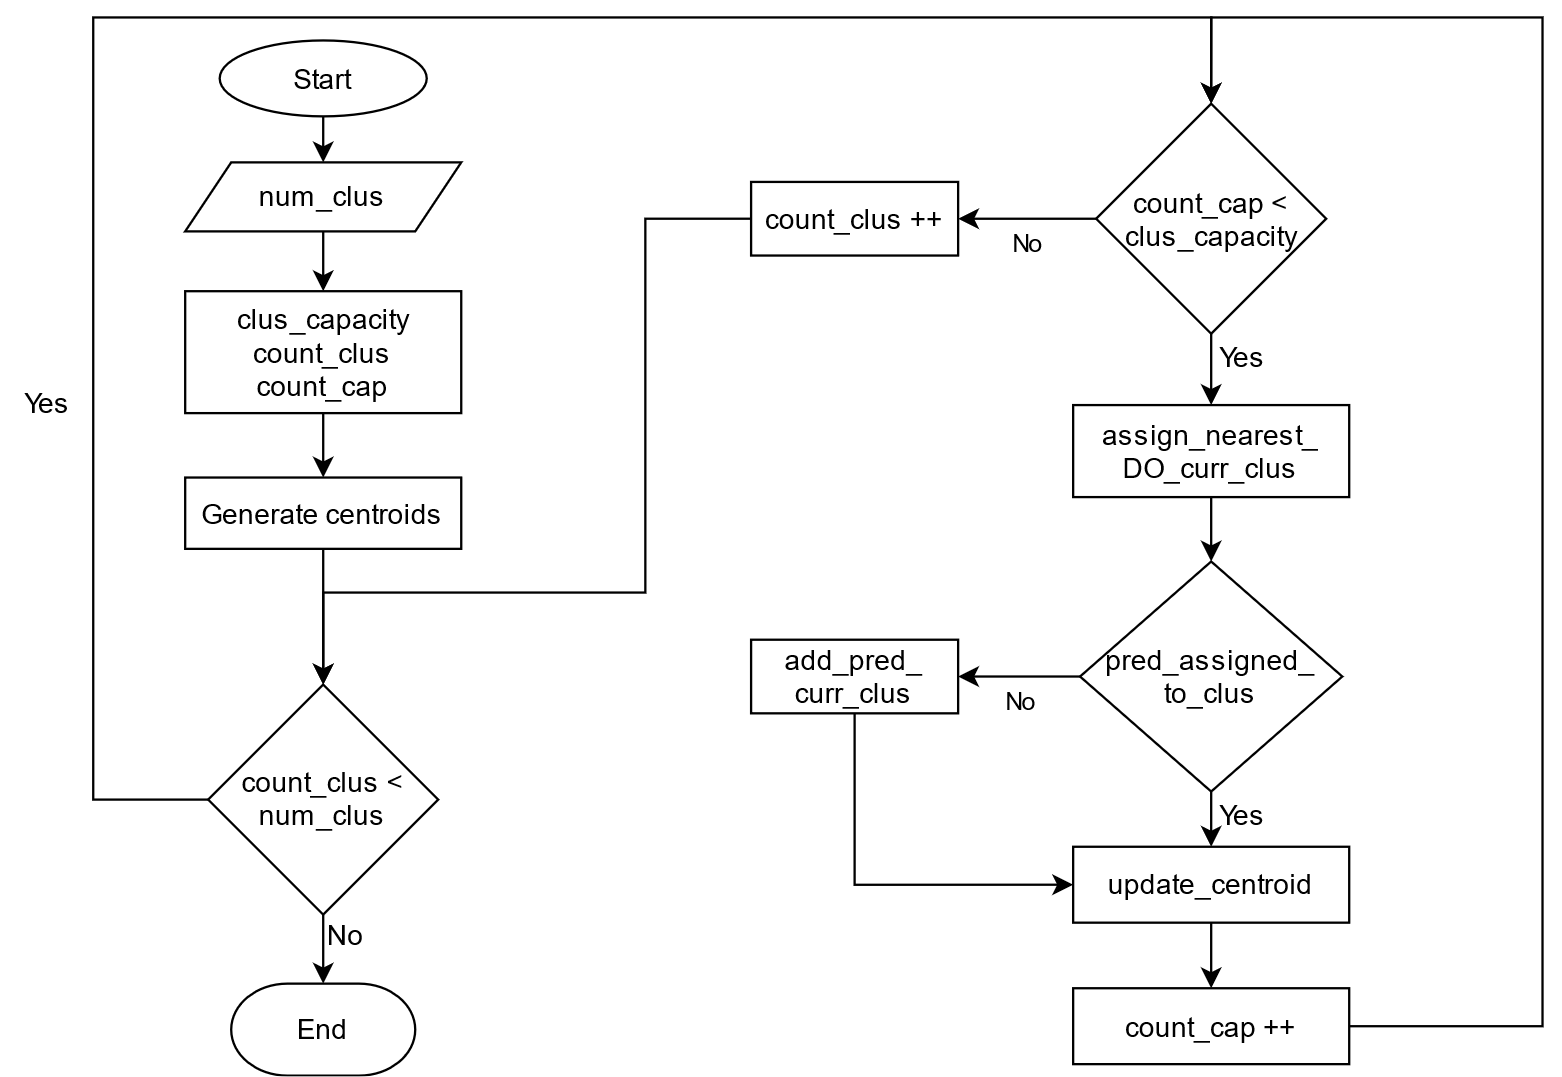
\includegraphics[width=\linewidth]{Flow_chart_9.png}
  \caption{Flowchart of the proposed Clustering Algorithm.}
  \label{fig1}
\end{figure}
\fi

In order to identify the most promising features for distance calculation among those introduced in the previous section,
we suggest the following forward selection principle:
% Our main procedure starts with the selection of a subset of the extracted features, which allows the clustering algorithm to compute the best possible time window assignments. 
% The procedure follows the forward feature selection principle:
start with a small set of features, perform decomposition by Algorithm~\ref{alg2},
and iteratively solve JSP instances.
Then, we evaluate the possible extensions by one more feature,
compare the quality of resulting schedules, and pick the best set of features. 
% and in every iteration extends it with one feature.
% Run the clustering algorithm on the new set of features and solve the obtained sequence of time windows. The subset of features resulting in the best possible solution quality is preserved and provided for extension in the next loop of the feature selection algorithm.
This process continues until either 
\begin{enumerate*}[label=\emph{(\roman*)}]
  \item all features are selected, or 
  \item any extension by another feature leads to solutions of lower quality.
\end{enumerate*}

%\newpage

\section{Evaluation Results}
\label{sec:eval}
We use randomly generated JSP instances
with $50$ jobs, $15$ machines, and $50\times 15=750$ operations,
part of which are known to be challenging for greedy and stochastic optimization techniques,
from Taillard's and Demirkol's benchmark suites \cite{taillard1993benchmarks,demirkol1998benchmarks} for the empirical evaluation of our approach.
%Many researchers have studied these instances and presented different approaches to solving them. We also developed different decomposition strategies to solve those. Therefore, it will be possible to measure the success/failure of our proposed model by comparing the results of the strategies developed in the past with those obtained from the proposed algorithm. 
For each instance, we extracted the $12$ features described in Section~\ref{sec:features}. In order to assess their impact % of the features
on the clustering and, consequently, the quality of schedules, we make fix use of the features \stfifo, \stmtwr, and \stest, which provide the starting times of operations obtained by
heuristic greedy search methods, as these three features promised to be informative
in preliminary experiments.
In contrast to that, considering the position of operations in jobs (\textit{OP}),
processing times (\textit{PT}), and jobs' time length (\textit{TLJ})
turned out to be counterproductive in our preliminary investigation,
so that we disregard such features in the following.
The six leftover features, i.e., remaining processing time (\textit{RPT}),
earliest starting time (\textit{EST}), machine load (\textit{ML})
as well as the waiting times \wtfifo, \wtmtwr, and \wtest
based on schedules computed by corresponding greedy algorithms,
are added and combined to feature sets as follows:
%\todo{The feature set
%\textit{\{ \stfifo, \stmtwr, \stest, RPT, EST, ML \}} would be logical as \textbf{F8},
%but it's missing.}
% we store and present the output of the feature selection step and results of the decomposition-based solving using the Answer Set Programming model developed in \cite{el2020job}.
% The feature selection algorithm was initialized with a simple combination that consists of $3$ features: \stfifo, \stmtwr, and \stest. The combinations of the selected features presented below. We neglected the rank of an operation and the time length of a job because they had negative impact results from the preliminary experiments.

\begin{enumerate}[label=]
\fontsize{9pt}{10pt}
\item \textbf{F1}\phantom{\textbf{0}} \textrightarrow{} \textit{\{ \stfifo, \stmtwr, \stest \}}
\item \textbf{F2}\phantom{\textbf{0}} \textrightarrow{} \textit{\{ \stfifo, \stmtwr, \stest, RPT \}}
\item \textbf{F3}\phantom{\textbf{0}} \textrightarrow{} \textit{\{ \stfifo, \stmtwr, \stest, EST \}} 
\item \textbf{F4}\phantom{\textbf{0}} \textrightarrow{} \textit{\{ \stfifo, \stmtwr, \stest, ML \}} 
\item \textbf{F5}\phantom{\textbf{0}} \textrightarrow{} \textit{\{ \stfifo, \stmtwr, \stest, RPT, EST \}}
\item \textbf{F6}\phantom{\textbf{0}} \textrightarrow{} \textit{\{ \stfifo, \stmtwr, \stest, RPT, ML \}} 
\item \textbf{F7}\phantom{\textbf{0}} \textrightarrow{} \textit{\{ \stfifo, \stmtwr, \stest, EST, ML \}}
\item  \textbf{F8}\phantom{\textbf{0}} \textrightarrow{} \textit{\{ \stfifo, \stmtwr, \stest, RPT, EST, ML \}}
\item \textbf{F9}\phantom{\textbf{0}} \textrightarrow{} \textit{\{ \stfifo, \stmtwr, \stest, \wtfifo, \wtmtwr, \wtest \}} 
\item \textbf{F10} \textrightarrow{} \textit{\{ \stfifo, \stmtwr, \stest, \wtfifo, \wtmtwr, \wtest, RPT \}} 
\item \textbf{F11} \textrightarrow{} \textit{\{ \stfifo, \stmtwr, \stest, \wtfifo, \wtmtwr, \wtest, EST \}} 
\item \textbf{F12} \textrightarrow{} \textit{\{ \stfifo, \stmtwr, \stest, \wtfifo, \wtmtwr, \wtest, ML \}}
\item \textbf{F13} \textrightarrow{} \textit{\{ \stfifo, \stmtwr, \stest, \wtfifo, \wtmtwr, \wtest, RPT, EST \}}
\item \textbf{F14} \textrightarrow{} \textit{\{ \stfifo, \stmtwr, \stest, \wtfifo, \wtmtwr, \wtest, RPT, ML \}}
\item \textbf{F15} \textrightarrow{} \textit{\{ \stfifo, \stmtwr, \stest, \wtfifo, \wtmtwr, \wtest, EST, ML \}}
\item \textbf{F16} \textrightarrow{} \textit{\{ \stfifo, \stmtwr, \stest, \wtfifo, \wtmtwr, \wtest, RPT, EST, ML \}}
\end{enumerate}

\begin{table}[bt]
  \begin{center}
    \caption{Solution quality comparison for different feature sets (Taillard's instances).}
    \label{tab4}
    \addtolength{\tabcolsep}{0.9pt}
    \begin{tabular}{|l|c|c|c|c|c|c|c|c|c|c|c|} \hline
%      & \multicolumn{11}{|c|}{\textbf{Instances}} \\ \cline{2-12}
      \textbf{Approach}   & TA51                           & TA52                           & TA53                           & TA54 & TA55                           & TA56                           & TA57                           & TA58 & TA59                           & TA60 & AVG  \\ \hline\hline
      \textbf{FIFO}        & 3549                           & 3339                           & \textbf{3160}              & \textbf{3218} & 3291               & 3325                           & 3654                           & \textbf{3299} & \textbf{3344}                           & \textbf{3129} & \textbf{3331} \\
      \textbf{MTWR}        & \textbf{3364}           & \textbf{3304}              & 3168                           & 3494 & \textbf{3237}                           & \textbf{3287}               & \textbf{3633}              & 3591 & 3394                           & 3257 & 3373 \\
      \textbf{Single-shot} & 3632                           & 3615                           & 3481                           & 3462 & 3552                           & 3610                           & 3778                           & 3718 & 3613                           & 3550 & 3601 \\ % \hline
%      \textbf{EST}         
      \textbf{Multi-shot}         & 3506                           & 3773                           & 3478                           & 3497 & 3482                           & 3605                           & 3753                           & 3731 & 3398                           & 3247 & 3547 \\ \hline
      \textbf{F1}          & 3506                           & 3277                           & 3382                           & 3414 & 3308                           & 3353                           & 3605                           & 3352 & 3453                           & 3483 & 3413 \\
      \textbf{F2}          & 3362                           & 3318                           & 3585                           & 3425 & 3441                           & 3380                           & 3573                           & 3412 & 3416                           & \textbf{3315} & 3423 \\
      \textbf{F3}          & 3324                           & 3330                           & 3347                           & 3425 & 3424                           & 3548                           & 3601                           & 3370 & 3301                           & 3617 & 3429 \\
      \textbf{F4}          & 3360                           & 3286                           & 3543                           & 3503 & 3319                           & 3270                           & 3583                           & 3509 & 3339                           & 3563 & 3428 \\
      \textbf{F5}          & 3346                           & 3243                           & 3517                           & 3397 & 3355                           & 3383                           & 3650                           & 3707 & 3508                           & 3591 & 3470 \\
      \textbf{F6}          & \textbf{3294} & 3275                           & 3250                           & 3265 & 3386                           & 3366                           & \textbf{3480} & \textbf{3324} & 3430                           & 3327 & \textbf{3340} \\
      \textbf{F7}          & 3328                           & 3226                           & 3338                           & 3353 & 3301                           & 3564                           & 3592                           & 3496 & 3352                           & 3399 & 3395 \\
      
      \textbf{F8}          & 3330                           & 3273                           & 3277                           & 3492 & 3375                           & 3469                           & 3760                           & 3410 & 3485                           & 3573 & 3444 \\

      \textbf{F9}          & 3588                           & 3397                           & 3251                           & 3563 & 3498                           & \textbf{3229} & 3621                           & 3517 & 3258                           & 3374 & 3430 \\
      \textbf{F10}          & 3588                           & 3373                           & 3522                           & 3443 & 3385                           & 3306                           & 3543                           & 3716 & 3381                           & 3526 & 3475 \\
      \textbf{F11}         & 3568                           & 3533                           & 3373                           & 3386 & 3530                           & 3362                           & 3608                           & 3644 & 3402                           & 3637 & 3504 \\
      \textbf{F12}         & 3514                           & 3256                           & 3585                           & 3352 & 3365                           & 3344                           & 3670                           & 3611 & \textbf{3145} & 3425 & 3427 \\
      \textbf{F13}         & 3682                           & 3494                           & \textbf{3143} & 3270 & 3309                           & 3332                           & 3632                           & 3471 & 3250                           & 3676 & 3426 \\
      \textbf{F14}         & 3624                           & 3505                           & 3427                           & 3236 & 3370                           & 3338                           & 3749                           & 3437 & 3253                           & 3659 & 3460 \\
      \textbf{F15}         & 3554                           & 3373                           & 3524                           & \textbf{3232} & 3385                           & 3483                           & 3573                           & 3365 & 3284                           & 3767 & 3454 \\
      \textbf{F16}         & 3509                           & \textbf{3184} & 3380                           & 3289 & \textbf{3218} & 3389                           & \textbf{3480} & 3481 & 3290                           & 3569 & 3379 \\ % \hline
      \textbf{Virtual Best} & \textbf{3294}                           & \textbf{3184} & \textbf{3143}                           & \textbf{3232} & \textbf{3218} & \textbf{3229}                           & \textbf{3480} & \textbf{3324} & \textbf{3145}                           & \textbf{3315} & \textbf{3256} \\
\hline
      \end{tabular}
  \end{center}
\end{table}

We utilized the above feature sets for partitioning the operations of JSP instances into $3$ clusters or time windows, respectively,
and then ran the multi-shot optimization approach introduced in~\cite{el2020job} for
$10$ minutes in total, i.e., $200$ seconds per time window,
on an
%\todo{Please check and update the machine and operating system setup.}
Intel\textsuperscript{\textregistered} Core\texttrademark{} i7-8650U CPU % \textsuperscript{\textregistered}
Dell Latitude 5590 machine under Windows 10.
%
The resulting quality of schedules in terms of the achieved makespan for each instance is reported in Table~\ref{tab4} and Table~\ref{tab5},
where the first four rows include the greedy FIFO and MTWR search methods supplied by the environment in~\cite{tagesc21a}
as well as single-shot and multi-shot pure ASP optimization, the latter taking earliest starting times instead of 
clustering for the decomposition into $3$ time windows,
for reference.
%
Regarding these reference methods, FIFO and MTWR are more or less on par, with a slight advantage of FIFO on Taillard's instances and an edge for MTWR on Demirkol's instances, 
indicated
by the average makespans given in the last column of each table.
While combinatorial optimization by neither single- nor multi-shot ASP 
solving is able to keep step within the time limit and leads to greater averages over all instances, the multi-shot pure ASP optimization approach turns out to be comparably robust
on half of the instances from Demirkol's benchmark suite,
which points out the critical impact of instance patterns.
%
\begin{table}[bt]
  \begin{center}
    \caption{Solution quality comparison for different feature sets (Demirkol's instances).}
    \label{tab5}
    \addtolength{\tabcolsep}{0.9pt}
    \begin{tabular}{|l|c|c|c|c|c|c|c|c|c|c|c|} \hline
%      & \multicolumn{11}{|c|}{\textbf{Instances}} \\ \cline{2-12}
      \textbf{Approach}  & DE31  & DE32 & DE33 & DE34 & DE35 & DE71 & DE72 & DE73 & DE74 & DE75 & AVG  \\ \hline

      \textbf{FIFO}  & \textbf{6817} & 6318 & \textbf{6029} & \textbf{6395} & \textbf{6409} & 9678 & 10349 & 9617 & 9847 & 9479 & 8094 \\
      \textbf{MTWR}  & 7155 & \textbf{6042} & 6819 & 6570 & 6881 & 7764 & 8407 & 8411 & 8321 & 7893 & \textbf{7426} \\
      \textbf{Single-shot} & 10370 & 10214 & 10064 & 10682 & 10203 & 6848 & 28369 & 32954 & 35325 & 6992 & 16202 \\
      \textbf{Multi-shot} & 10318  & 9522  & 9785 & 10775 & 10398 & \textbf{6492}  & \textbf{6935} & \textbf{7202} & \textbf{7128}  & \textbf{6243} & 8480 \\ \hline
      \textbf{F1}  & 8488  & 8325  & 7831 & 8356 & 8088 & 8593  & 7188 & 7826 & 6611 & 7662 & 7897 \\
      \textbf{F2}  & 8440  & 8298  & \textbf{7663} & 8479 & 7986 & 6994  & 7606 & 7209 & 6627 & 7069 & 7637 \\
      \textbf{F3}  & 8234  & 8401  & 8037 & 8444 & 7780 & \textbf{6590}  & 7785 & 7302 & 6690 & 7051 & 7631 \\
      \textbf{F4}  & 7991  & 8589  & 7996 & 8471 & 8207 & 8091  & 7834 & 6972 & 6708 & 6859 & 7771 \\
      \textbf{F5}  & 8164  & 8103  & 7835 & 8482 & 7802 & 6807  & 8357 & 7328 & 6774 & 7192 & 7684\\
      \textbf{F6}  & \textbf{7709} & 8265 & 7795 & 8475 & \textbf{7678}  & 6611 & 6708 & 7030 &6569 & 6867 & \textbf{7371} \\
      \textbf{F7}  & 8268  & 8553  & 7892 & 8359 & 8032 & 7603  & 6855 & 7223 & 6609 & 7200 & 7659 \\
      \textbf{F8}  & 8873 & 8879 & 8201 & 9126 & 7982 & 6843 & 7971 & 7106 & 7545 & 6970 & 7950 \\
      \textbf{F9}  & 8500  & 8185  & 8533 & 8772 & 8535 & 6726 & 6518& 7130 & 6592 & 7262 & 7675 \\
      \textbf{F10}  & 8322  & 8119  & 8433 & 8910 & 8233 & 6868 & 6764 & 7183 & 6267 & 7459 & 7656 \\
      \textbf{F11} & 8617  & 8383  & 8614 & 8755 & 7969 & 7587 & \textbf{6512} & \textbf{6762}& 6505 & 7376 & 7708 \\
      \textbf{F12} & 8400  & 8124  & 8043 & \textbf{8185} & 8799 & 7849 & 6618 & 6876 & 6397 & 7746 & 7704 \\
      \textbf{F13} & 8916 & 8343  & 8441 & 8331 & 8153 & 7464 & 6757 & 6994 & 6434 & 6961 & 7679 \\
      \textbf{F14} & 8392  & \textbf{7937} & 7943 & 8375 & 8049 & 7310 & 7703 & 6827 & \textbf{6126} & 6893 & 7555 \\
      \textbf{F15} & 8412  & 8210  & 8117 & 8563 & 9068 & 7853 & 6968 & 6909 & 6350  & 7011 & 7746 \\
      \textbf{F16} & 8184 & 8150 & 8295 & 8721 & 8003 & 6997 & 7156 & 6991 & 6355 & \textbf{6584} & 7544 \\ 
      \textbf{Virtual Best} & \textbf{7709} & \textbf{7937} & \textbf{7663} & \textbf{8185} & \textbf{7678} & \textbf{6590} & \textbf{6512} & \textbf{6762} & \textbf{6126} & \textbf{6584} & \textbf{7175} \\
\hline
      \end{tabular}
  \end{center}
\end{table}

Among our feature sets for clustering, in preparation of multi-shot optimization by ASP,
we do not identify any clear winner dominating over all instances.
However, the feature sets \textbf{F2}, \textbf{F6}, \textbf{F11}, \textbf{F12}, \textbf{F13}, \textbf{F14}, and \textbf{F16}
yield significant makespan improvements relative to the other alternatives on particular instances.
This means that considering the features \textit{RPT}, \textit{EST}, \textit{ML}, or
\wtfifo, \wtmtwr, and \wtest in addition to starting times \stfifo, \stmtwr, and \stest by
greedy algorithms is beneficial, while the particular combination of features achieving best schedules varies.
Moreover, our clustering method for JSP instance decomposition outperforms (multi-shot) pure ASP optimization,
and specific feature sets are ahead of the greedy FIFO and MTWR algorithms on seven out of ten Taillard's instances as well as half of Demirkol's instances,
as indicated by the virtual best clustering results in the last row of Table~\ref{tab4}
and Table~\ref{tab5}.
Notably, the feature set \textbf{F6} leads to the shortest average makespans for
our cluster-wise JSP solving approach on both kinds of instances, comes close to
FIFO on Taillard's and is most robust on Demirkol's instances, but the
virtual best clustering results still improve significantly.
% In Table~\ref{tab5}, the feature sets outperformed the greedy on only three out of ten instances. However, feature set \textbf{F6} provided the best obtained average. 
We thus conclude that the instance decomposition by clustering can empower iterative combinatorial optimization
to find better schedules than greedy algorithms in a short amount of time, where alternative feature sets deserve
attention and trying several of them in parallel seems advisable.

% Table~\ref{tab4} shows the selected features and the performance of each combination for solving benchmark instances of 50 jobs and 15 machines \cite{taillard1993benchmarks}. The first column shows the approaches used for solving the problem in the literature in addition to the combinations of features considered by our feature selection algorithm. The next columns represent the instances of our benchmark set except for the last column, which shows the average of each approach through the whole benchmark set. The first $4$ rows in the table show the values of each makespan obtained by heuristics; FIFO, MTWR, and EST with a single and multi-shot ASP solving. We can conclude that FIFO and MTWR provided the best results compared to the other two heuristics. However for the features combinations, the sets (\textbf{F6}, \textbf{F8}, \textbf{F11}, \textbf{F12} and \textbf{F15}) provided good results according to the cost function in the most cases especially with combinations (\textbf{F6} and \textbf{F15}). It means that the most important features extracted from the problem itself and have a positive impact on the performance are \textit{Remaining Processing Time, Machine Load and Earliest Starting Time}. Also, the information obtained from the solutions of the other heuristics, like \textit{Starting Time} and \textit{Waiting Time}, led our algorithm to better decomposition for the problem at hand. More specifically, combining \textit{Remaining Processing Time} with \textit{Machine Load} provides a good decomposition with/without \textit{Waiting Time} attributes obtained by the other heuristics. In a few instances, our proposed method did not outperform other heuristics. However, in general, the best average makespan of the other approaches was $3331$ by FIFO, and the average makespan of our feature selection algorithm was $3256$. Therefore, the feature selection algorithm outperformed other heuristics in the literature by efficiently combining different heuristic information using clustering and feature selection.

\section{Related Work}
\label{sec:literature}

Data mining approaches~\cite{ismail2012production} have been extensively proposed and applied to generate % so-called
dispatching rules~\cite{blackstone1982state} for scheduling problems.
Unlike combinatorial and stochastic optimization methods, dispatching rules do not take
complete schedules into account, but address the prioritization of operations for making
local allocation decisions by greedy scheduling algorithms.
In addition to Earliest Starting Time (EST), First-In-First-Out (FIFO), and
Most Total Work Remaining (MTWR), which we also use for obtaining starting times as features,
common dispatching rules include Last-In-First-Out (LIFO) and policies incorporating
Job Length (JL) in terms of the number of operations as well as further features
like those described in Section~\ref{sec:features}:
Operation Position (OP), Processing Time (PT), Remaining Processing Time (RPT), 
Time Length of a Job (TLJ), and Machine Load (ML).
While dispatching rules enable an efficient operation allocation,
even under real-time conditions, the quality of their decisions heavily depends on the
problem instances under consideration, where data mining techniques come in to
improve over tedious and ad hoc manual tuning.

The approach of~\cite{koonce2000using} incorporates data mining methods,
using OP, PT, RPT, and ML as features, for generating dispatching rules that approximate
operation priorities found in schedules optimized by means of a genetic algorithm.
On randomly generated test instances of comparably small size, i.e., $36$ operations
per instance, the generated dispatching rules were shown to outperform greedy search
with shortest PT as a rigid criterion for making allocation decisions.
Genetic algorithms are also utilized in~\cite{harrath2002genetic} to obtain
promising solutions for JSP instances and extract features to consider for the
construction of dispatching rules.
The specifically generated three-tiered policy comprises shortest PT, smallest JL, and longest RPT as
dispatching criteria in the order of significance.
Note that such a composite dispatching rule needs to reconstructed from scratch when
new features or problem instances are analyzed, while our constrained clustering method
can readily be applied to different instance or feature sets, respectively.

Beyond static scheduling, dynamic JSP~\cite{french82a} deals with events, such as 
the release of new jobs or sudden machine breakdowns, along with rescheduling or
updating dispatching rules, respectively.
In analogy to the static setting,
the processing approach of~\cite{shahzad2010discovering} applies tabu search to
training instances and generates allocation policies approximating the optimized
complete schedules based on features like EST, PT, and RPT of operations.
Applied in the dynamic JSP setting, the dispatching rules obtained by means of data mining
were shown to yield better or comparable performance to rigid allocation strategies from the
literature.
A rescheduling approach combining Variable Neighborhood Search (VNS)
with K-Means clustering is presented in~\cite{adibi2014clustering},
where clusters are updated to reconfigure the VNS on each event.
The performance of this combined rescheduling strategy in the dynamic JSP setting turned out
to be better than pure VNS and greedy algorithms with the FIFO, LIFO, or
shortest PT allocation policy.

The integration of dispatching rules generated with data mining techniques
into stochastic optimization in~\cite{nasiri2019data} works by
running a greedy algorithm called ``assignment procedure'' to obtain promising
JSP solutions and mine dispatching rules approximating them.
But instead of relying on the dispatching rules alone for computing optimized
schedules or performing efficient operation allocation on new instances,
the high-quality draft solutions from greedy search with the dispatching rules
are taken as inputs to population-based stochastic optimization.
This metaheuristic optimization was shown to yield improved outcomes when launched
with schedules generated by means of suitable dispatching rules rather than with
a randomly generated initial population.

Similarities of our cluster-wise JSP solving approach to the discussed methods include
that we apply (fixed) dispatching rules to extract the starting times of operations
in corresponding schedules as instance features.
Notably, the constrained clustering algorithm in Section~\ref{sec:method} can readily
be applied to arbitrary feature sets for decomposing the operations of JSP instances
into balanced time windows, i.e., our clustering method does not presuppose tuning to
specific instance or feature sets under consideration.
The iterative combinatorial optimization by time windows can be viewed as a trade-off
between efficient dispatching rules, aiming to optimize local allocation decisions by
prioritizing operations, and the stochastic or combinatorial optimization of
complete schedules for problem instances.
While instance size and complexity can make the search for optimal solutions
with state-of-the-art solvers for ASP, Mixed Integer Programming, or Constraint Programming
prohibitive~\cite{coltep19a,zhang2010hybrid},
successful % their real-world 
application areas in scheduling include, e.g.,
industrial printing~\cite{balduccini11a},
team-building~\cite{rigralmaliiile12a},
shift design~\cite{abgemuscwo15c},
course timetabling~\cite{bainkaokscsotawa18a},
lab resource allocation~\cite{frscel21a},
and
medical treatment planning~\cite{dogagrmamopo21a}.

% In this section, we review some of the most related work using data mining approaches employed to solve scheduling problems. Over the last decades, solving the scheduling problem has attracted the interest of many researchers. The main idea of data mining in these applications is to explore the patterns from the obtained solutions by some heuristics and then develop decision rules that approximate the order of the operations in each machine \cite{ismail2012production}. More precisely, it aims to get an order of all operations in the given instance according to their characteristics.

% Data mining methodologies were applied to explore the patterns in data generated by genetic algorithms in \cite{koonce2000using}. This work aimed to generate rules determining the priority for each job. The authors solved the scheduling problem using a genetic algorithm and derived dispatching rules that considered characteristics like the rank of operations, processing time, machine load, and remaining processing time. The evaluation of the obtained rules was done on previously unused random instances. Obtained results show that the generated rules were able to outperform the shortest processing time heuristic. One of the drawbacks is that the problem instances considered contain only 36 operations, i.e., considered JSP instances were relatively small.

% The authors in \cite{harrath2002genetic} also implemented a genetic algorithm to construct and analyze solutions of JSP instances for the feature extraction for the suggested dispatching rule. In particular, the approach uses processing time, job length, remaining processing time, the rank of the operation, and machine load. The authors preprocessed the data by converting it from quantitative into qualitative representation, which was then used to build a generic model for scheduling problems as follows: First, the authors sorted the operations share the same machine according to processing time. Then, if two or more operations have the same processing time, the heuristic preferred a job with the smallest length. Finally, if the jobs have the same length, the remaining processing time heuristic was used as a tie-breaker. In opposite, our approach does not depend on a set of features extracted from an instance. New features can easily be included in the set of observations and considered by the clustering method.

% In addition to the work focusing on static JSP, there are approaches using data mining methods for dynamic JSP. For instance, \cite{shahzad2010discovering} presents new dispatching rules for JSP aiming to minimize makespan and which process a given JSP instance as follows: 
% First, a scheduling instance is solved using Tabu Search and the obtained solutions are used as a training set to get a rule-set capable of approximating efficient solutions. This approach considers features like EST, the difference in remaining processing time for a job, and the difference in the processing time of two operations, to create a rule-set for dispatching the operations. The experiments showed that the results of mined rule-set are superior or comparable to the heuristics in the literature.

% The variable neighborhood search (VNS) is combined with the k-Means algorithm to address Dynamic JSP \cite{adibi2014clustering}. The proposed algorithm depends on extracting information from the problem's input data when an event, like a machine breakdown or an addition of a new job, occurs. At any rescheduling point, cluster analysis is performed to replace jobs according to their distances. In other words, a job that belongs to a farther cluster has a greater probability to be selected in making a new adjacent than the other belonging to a closer cluster. The proposed method was compared to VNS and some common heuristics using a simulated job shop. the results indicated that the performance of the proposed model is better than the others, including heuristics like FIFO, LIFO, and SPT.

% Another study has presented a data mining approach to generate an initial population for population-based heuristics/metaheuristics to solve JSP \cite{nasiri2019data}. They extracted information from optimal or near-optimal solutions obtained by a heuristic procedure called "Assignment Procedure" to build decision rules to determine the priority of the operations. Once the rules are extracted, the initial solution is generated using these rules. To evaluate the performance of the proposed method, they performed a series of computational experiments on several test instances. The results showed that the proposed method with data mining generated initial population outperforms the methods with randomly generated initial population.

% From the literature, we have found that most of the studies which used data mining techniques aimed to extract some features either from the problem instances or solutions obtained by some heuristics to build a decision-rules to order the operations assigned to a machine. In most cases, these approaches depend on the set of extracted features and cannot add new or remove the existing ones. Our approach is completely independent of the underlying set of features and, therefore, has broader and more flexible applications.


\section{Conclusions}
\label{sec:conclusions}
Data mining and machine learning are of wide interest in scientific, business, and further fields. % In order to increase productivity and decrease the operation cost, there should be high-quality schedules to be used.
Our work investigates data mining and clustering methods to optimize solutions for the Job-shop Scheduling Problem within short solving times.
The idea is to associate clusters of operations with time windows subject to iterative combinatorial optimization, eventually leading to a complete schedule.
In contrast to usual clustering tasks, however,
the time windows need to take the sequence of operations in a job into account,
and the number of operations per cluster should also be balanced for partitioning
a given problem instance into time windows of roughly similar solving complexity.
We have thus devised a novel constrained clustering method that takes both concerns
into account for gathering operations with similar feature values in a consistent and
balanced way.
Our experiments show that the decomposition into time windows obtained by clustering
usually leads to significantly improved outcomes of multi-shot ASP solving in comparison
to taking earliest starting times as simple (and consistent) partitioning criterion.
While no single feature set for clustering turns out to be strictly more successful than greedy search
with FIFO or MTWR allocation policy, schedules of comparable or better quality can be found
with some feature set in the given solving time for most instances.
Moreover, the iterative combinatorial optimization by time windows helps to increase
the robustness of schedules obtained for different kinds of instances.

While search for optimal solutions is beyond reach due to the size and complexity of
practical scheduling applications,
reliably computing high-quality approximations is an important subject of future work.
This includes automatic methods for deciding about the features to consider for
partitioning operations into clusters, i.e., determining whether an eligible feature is
informative or noisy, respectively.
As we can hardly expect that even moderately sized time windows can be solved to
optimality in a short amount of time or eventual optimization criteria values be
accurately predicted from solutions for sub-problems,
it can still be worthwhile to incorporate measures allowing for corrections of 
partitioning decisions, which could consist of overlapping time windows to enable
revisions or dynamically relaunching the clustering algorithm wrt.\ computed
partial schedules.
Instead of obtaining features by greedy search methods only, we may also take
the outcomes of one or several multi-shot optimization runs into account as
features for another clustering and solving round until a fixpoint without
further improvement is reached.
That is, there are various opportunities to extend our approach in the future,
where going beyond the classical Job-shop Scheduling Problem, e.g., by
considering flexible resource allocations or partially ordered operations,
can also be of interest for practical application scenarios.

% The first issue in this work is to explore the knowledge in good schedules and try to use this knowledge to get more efficient schedules. We extracted some features from the problem at hand and other features from schedules obtained by heuristics. The second issue is finding a powerful way to decompose the problem into windows where each cluster is a window and solve them sequentially. In order to split the problem, we proposed a constrained clustering algorithm considering the precedence constraints of the JSP. We tested our model on benchmark instances, and the results showed that the performance of the proposed model outperforms other heuristics FIFO, MTWR, and EST in the most cases; and some attributes like (\textit{Starting Time, Waiting Time, Remaining Processing Time, and Machine Load}) played an important role to split the operations in a good way. There are several ways to extend this study. Firstly, solve bigger instances and others in a real-life application in which more features could be extracted. Secondly, develop other clustering algorithms to split the problem more efficiently and get better results.

% \bibliographystyle{splncs04}
% \bibliography{references}
\begin{thebibliography}{10}
\providecommand{\url}[1]{\texttt{#1}}
\providecommand{\urlprefix}{URL }
\providecommand{\doi}[1]{https://doi.org/#1}

\bibitem{abgemuscwo15c}
Abseher, M., Gebser, M., Musliu, N., Schaub, T., Woltran, S.: Shift design with
  answer set programming. Fundamenta Informaticae  \textbf{147}(1),  1--25
  (2016)

\bibitem{adibi2014clustering}
Adibi, M., Shahrabi, J.: A clustering-based modified variable neighborhood
  search algorithm for a dynamic job shop scheduling problem. International
  Journal of Advanced Manufacturing Technology  \textbf{70}(9-12),  1955--1961
  (2014)

\bibitem{al2017job}
Al-Ashhab, M., Munshi, S., Oreijah, M., Ghulman, H.: Job shop scheduling using
  mixed integer programming. International Journal Of Modern Engineering
  Research  \textbf{7}(3),  2:23--2:29 (2017)

\bibitem{baker1974introduction}
Baker, K.: Introduction to Sequencing and Scheduling. John Wiley \& Sons (1974)

\bibitem{balduccini11a}
Balduccini, M.: Industrial-size scheduling with {ASP}+{CP}. In: Proceedings of
  the Eleventh International Conference on Logic Programming and Nonmonotonic
  Reasoning (LPNMR'11), pp. 284--296. Springer-Verlag (2011)

\bibitem{bainkaokscsotawa18a}
Banbara, M., Inoue, K., Kaufmann, B., Okimoto, T., Schaub, T., Soh, T., Tamura,
  N., Wanko, P.: teaspoon: Solving the curriculum-based course timetabling
  problems with answer set programming. Annals of Operations Research
  \textbf{275}(1),  3--37 (2019)

\bibitem{bengio2020machine}
Bengio, Y., Lodi, A., Prouvost, A.: Machine learning for combinatorial
  optimization: A methodological tour d'horizon. European Journal of
  Operational Research  \textbf{290}(2),  405--421 (2021)

\bibitem{blackstone1982state}
Blackstone, J., Phillips, D., Hogg, G.: A state-of-the-art survey of
  dispatching rules for manufacturing job shop operations. International
  Journal of Production Research  \textbf{20}(1),  27--45 (1982)

\bibitem{DBLP:journals/jim/CalisB15}
{\c{C}}alis, B., Bulkan, S.: A research survey: Review of {AI} solution
  strategies of job shop scheduling problem. Journal of Intelligent
  Manufacturing  \textbf{26}(5),  961--973 (2015)

\bibitem{chaudhry2016research}
Chaudhry, I., Khan, A.: A research survey: Review of flexible job shop
  scheduling techniques. International Transactions in Operational Research
  \textbf{23}(3),  551--591 (2016)

\bibitem{coltep19a}
{Da Col}, G., Teppan, E.: Industrial size job shop scheduling tackled by
  present day {CP} solvers. In: Proceedings of the Twenty-fifth International
  Conference on Principles and Practice of Constraint Programming (CP'19), pp.
  144--160. Springer-Verlag (2019)

\bibitem{demirbilek2019dynamically}
Demirbilek, M., Branke, J., Strauss, A.: Dynamically accepting and scheduling
  patients for home healthcare. Health Care Management Science  \textbf{22}(1),
   140--155 (2019)

\bibitem{demirkol1998benchmarks}
Demirkol, E., Mehta, S., Uzsoy, R.: Benchmarks for shop scheduling problems.
  European Journal of Operational Research  \textbf{109}(1),  137--141 (1998)

\bibitem{ding2020unified}
Ding, H., Xu, J.: A unified framework for clustering constrained data without
  locality property. Algorithmica  \textbf{82}(4),  808--852 (2020)

\bibitem{dogagrmamopo21a}
Dodaro, C., Galat{\`{a}}, G., Grioni, A., Maratea, M., Mochi, M., Porro, I.: An
  {ASP}-based solution to the chemotherapy treatment scheduling problem. Theory
  and Practice of Logic Programming  \textbf{First
  View}(\url{https://doi.org/10.1017/S1471068421000363}),  1--17 (2021)

\bibitem{el2020job}
El-Kholany, M., Gebser, M.: Job shop scheduling with multi-shot {ASP}. In:
  Proceedings of the Fourth Workshop on Trends and Applications of Answer Set
  Programming (TAASP'20).
  \url{http://www.kr.tuwien.ac.at/events/taasp20/papers/TAASP_2020_paper_4.pdf}
  (2020)

\bibitem{Forgy1965ClusterAO}
Forgy, E.: Cluster analysis of multivariate data: Efficiency versus
  interpretability of classifications. Biometrics  \textbf{21},  768--769
  (1965)

\bibitem{frscel21a}
Francescutto, G., Schekotihin, K., El{-}Kholany, M.: Solving a multi-resource
  partial-ordering flexible variant of the job-shop scheduling problem with
  hybrid {ASP}. In: Proceedings of the Seventeenth European Conference on
  Logics in Artificial Intelligence (JELIA'21), pp. 313--328. Springer-Verlag
  (2021)

\bibitem{french82a}
French, S.: Sequencing and Scheduling: An Introduction to the Mathematics of
  the Job-shop. John Wiley \& Sons (1982)

\bibitem{garey1976complexity}
Garey, M., Johnson, D., Sethi, R.: The complexity of flowshop and jobshop
  scheduling. Mathematics of Operations Research  \textbf{1}(2),  117--129
  (1976)

\bibitem{gekakasc17a}
Gebser, M., Kaminski, R., Kaufmann, B., Schaub, T.: Multi-shot {ASP} solving
  with clingo. Theory and Practice of Logic Programming  \textbf{19}(1),
  27--82 (2019)

\bibitem{harrath2002genetic}
Harrath, Y., Chebel-Morello, B., Zerhouni, N.: A genetic algorithm and data
  mining based meta-heuristic for job shop scheduling problem. In: Proceedings
  of the IEEE International Conference on Systems, Man and Cybernetics
  (SMC'02). IEEE (2002)

\bibitem{ismail2012production}
Ismail, R., Othman, Z., Bakar, A.: A production schedule generator framework
  for pattern sequential mining. In: Proceedings of the Seventh International
  Conference on Computing and Convergence Technology (ICCCT'12), pp. 784--788.
  IEEE (2012)

\bibitem{janakbhai2021blockchain}
Janakbhai, N., Saurin, M., Patel, M.: Blockchain-based intelligent
  transportation system with priority scheduling. In: Data Science and
  Intelligent Applications, pp. 311--317. Springer-Verlag (2021)

\bibitem{jones1998survey}
Jones, A., Rabelo, L., Sharawi, A.: Survey of job shop scheduling techniques.
  National Institute of Standards and Technology  \textbf{Encyclopedia of
  Electrical and Electronics
  Engineering}(\url{https://tsapps.nist.gov/publication/get_pdf.cfm?pub_id=821200})
  (1998)

\bibitem{koonce2000using}
Koonce, D., Tsai, S.: Using data mining to find patterns in genetic algorithm
  solutions to a job shop schedule. Computers \& Industrial Engineering
  \textbf{38}(3),  361--374 (2000)

\bibitem{lenstra1979computational}
Lenstra, J., Rinnooy~Kan, A.: Computational complexity of discrete optimization
  problems. Annals of Discrete Mathematics  \textbf{4},  121--140 (1979)

\bibitem{meng2020mixed}
Meng, L., Zhang, C., Ren, Y., Zhang, B., Lv, C.: Mixed-integer linear
  programming and constraint programming formulations for solving distributed
  flexible job shop scheduling problem. Computers \& Industrial Engineering
  \textbf{142},  Article 106347 (2020)

\bibitem{nasiri2019data}
Nasiri, M., Salesi, S., Rahbari, A., Meydani, N., Abdollai, M.: A data mining
  approach for population-based methods to solve the {JSSP}. Soft Computing
  \textbf{23}(21),  11107--11122 (2019)

\bibitem{nouiri2018effective}
Nouiri, M., Bekrar, A., Jemai, A., Niar, S., Ammari, A.: An effective and
  distributed particle swarm optimization algorithm for flexible job-shop
  scheduling problem. Journal of Intelligent Manufacturing  \textbf{29}(3),
  603--615 (2018)

\bibitem{ovacik2012decomposition}
Ovacik, I., Uzsoy, R.: Decomposition Methods for Complex Factory Scheduling
  Problems. Kluwer Academic Publishers (1997)

\bibitem{pezzella2008genetic}
Pezzella, F., Morganti, G., Ciaschetti, G.: A genetic algorithm for the
  flexible job-shop scheduling problem. Computers \& Operations Research
  \textbf{35}(10),  3202--3212 (2008)

\bibitem{rigralmaliiile12a}
Ricca, F., Grasso, G., Alviano, M., Manna, M., Lio, V., Iiritano, S., Leone,
  N.: Team-building with answer set programming in the {G}ioia-{T}auro seaport.
  Theory and Practice of Logic Programming  \textbf{12}(3),  361--381 (2012)

\bibitem{schoenfelder2020nurse}
Schoenfelder, J., Bretthauer, K., Wright, D., Coe, E.: Nurse scheduling with
  quick-response methods: Improving hospital performance, nurse workload, and
  patient experience. European Journal of Operational Research
  \textbf{283}(1),  390--403 (2020)

\bibitem{shahzad2010discovering}
Shahzad, A., Mebarki, N.: Discovering dispatching rules for job shop scheduling
  problem through data mining. In: Proceedings of the Eighth International
  Conference of Modeling and Simulation (MOSIM'10).
  \url{https://www.academia.edu/3068769/DISCOVERING_DISPATCHING_RULES_FOR_JOB_SHOP_SCHEDULING_PROBLEM_THROUGH_DATA_MINING}
  (2010)

\bibitem{singer2001decomposition}
Singer, M.: Decomposition methods for large job shops. Computers \& Operations
  Research  \textbf{28}(3),  193--207 (2001)

\bibitem{SOTSKOV1995237}
Sotskov, Y., Shakhlevich, N.: {NP}-hardness of shop-scheduling problems with
  three jobs. Discrete Applied Mathematics  \textbf{59}(3),  237--266 (1995)

\bibitem{taillard1993benchmarks}
Taillard, E.: Benchmarks for basic scheduling problems. European Journal of
  Operational Research  \textbf{64}(2),  278--285 (1993)

\bibitem{tagesc21a}
Tassel, P., Gebser, M., Schekotihin, K.: A reinforcement learning environment
  for job-shop scheduling. In: Proceedings of the ICAPS 2021 Workshop on
  Planning and Reinforcement Learning (PRL'21).
  \url{https://prl-theworkshop.github.io/prl2021/papers/PRL2021_paper_9.pdf}
  (2021)

\bibitem{uzsoy2000performance}
Uzsoy, R., Wang, C.: Performance of decomposition procedures for job shop
  scheduling problems with bottleneck machines. International Journal of
  Production Research  \textbf{38}(6),  1271--1286 (2000)

\bibitem{DBLP:journals/informs/VaessensAL96}
Vaessens, R., Aarts, E., Lenstra, J.: Job shop scheduling by local search.
  INFORMS Journal on Computing  \textbf{8}(3),  302--317 (1996)

\bibitem{wagstaff2001constrained}
Wagstaff, K., Cardie, C., Rogers, S., Schr{\"{o}}dl, S.: Constrained k-means
  clustering with background knowledge. In: Proceedings of the Eighteenth
  International Conference on Machine Learning (ICML'01), pp. 577--584. Morgan
  Kaufmann (2001)

\bibitem{wang2019routing}
Wang, H.: Routing and scheduling for a last-mile transportation system.
  Transportation Science  \textbf{53}(1),  131--147 (2019)

\bibitem{zhai2014decomposition}
Zhai, Y., Liu, C., Chu, W., Guo, R., Liu, C.: A decomposition heuristics based
  on multi-bottleneck machines for large-scale job shop scheduling problems.
  Journal of Industrial Engineering and Management  \textbf{7}(5),  1397--1414
  (2014)

\bibitem{zhang2019framework}
Zhang, H., Basu, S., Davidson, I.: A framework for deep constrained clustering:
  Algorithms and advances. In: Proceedings of the Joint European Conference on
  Machine Learning and Knowledge Discovery in Databases (ECML/PKDD'19), pp.
  57--72. Springer-Verlag (2019)

\bibitem{zhang2010hybrid}
Zhang, R., Wu, C.: A hybrid approach to large-scale job shop scheduling.
  Applied Intelligence  \textbf{32}(1),  47--59 (2010)

\end{thebibliography}


\end{document}
